\documentclass{article}
\usepackage{graphicx}
\usepackage{math_blog}

\title{Construction of Brownian Motion and Stochastic Processes}
\author{Anqiao Ouyang}
\date{July 29, 2025}

\newcommand{\Title}{Construction of Brownian Motion and Stochastic Processes}
\newcommand{\Column}{Stochastic Differential Equations I}
\newcommand{\Author}{Anqiao Ouyang}

\begin{document}

\maketitle

\section{Introduction}

When modeling uncertainty in the real world, traditional ordinary differential equations (ODEs) often fall short. We need mathematical tools that can handle randomness, leading us to stochastic differential equations (SDEs). As the first article in this series, we will systematically introduce the foundational aspects from a mathematical perspective. We will define what a stochastic process is, explain the concepts of filtration and adaptability, and then delve into Brownian motion as a core example. Subsequently, we will understand the rigorous logic behind Brownian motion as a driving term in SDEs and learn how it is constructed.

Readers are expected to have a basic mathematical background, primarily including high school calculus, basic probability theory (especially familiarity with probability spaces, random variables, distributions, and independence), and an initial understanding of measure theory. Although this article will strive to guide understanding through intuitive explanations, readers who wish to gain a deeper grasp of the underlying logical structure are encouraged to review or supplement their foundational knowledge as needed during the reading process.

\section{Basic Definitions of Stochastic Processes}

\subsection{Formal Definition}

\begin{definition}[Stochastic Process]
Let $(\Omega, \mathcal{F}, \mathbb{P})$ be a probability space, and let $T$ be an index set for time (e.g., $T = \mathbb{N}$ or $T = [0, \infty)$), with state space $\mathbb{R}^d$. If for each $t \in T$, the mapping $X_t : \Omega \to \mathbb{R}^d$ is an $\mathcal{F}$-measurable random variable, then the collection $\{X_t\}_{t \in T}$ is called a stochastic process taking values in $\mathbb{R}^d$.
\end{definition}

Intuitively, a stochastic process is a collection of random variables that evolve over time. Unlike a single random variable, it captures how randomness accumulates and unfolds through time, shifting focus from isolated outcomes to the evolution of the process itself. For each $\omega \in \Omega$, we obtain a sample path $t \mapsto X_t(\omega)$, which describes the complete trajectory of the system in a particular scenario. For instance, in financial markets, a stock price can be modeled as a real-valued stochastic process in continuous time.

The definition should feel fairly intuitive, right? That said, to further develop the theory, intuition alone won't suffice, and we must also study some classical stochastic processes and understand their structure and properties.

\subsection{Poisson Process}

To briefly review, the Poisson distribution is commonly used to describe the number of sparse and independent events occurring within a fixed time interval, where $\lambda$ represents the average number of occurrences in that interval. For example, if we receive an average of 3 phone calls per minute, then the probability of receiving $k$ calls in a given minute follows a Poisson distribution with parameter $\lambda = 3$.

\begin{definition}[Poisson Distribution]
Let $\lambda > 0$ be a given parameter. A discrete random variable $N$ is said to follow a Poisson distribution with parameter $\lambda$, denoted by $N \sim \text{Poisson}(\lambda)$, if its probability mass function is:
\[
\mathbb{P}(N = k) = \frac{\lambda^k e^{-\lambda}}{k!}, \quad \forall k \in \mathbb{N}_0.
\]
\end{definition}

We extend the concept of the Poisson distribution into a continuous-time framework, such that the increments of the process over time intervals follow Poisson distributions with appropriate parameters. This yields what we call a Poisson process.

The Poisson process is a classical model used to represent a sequence of discrete events occurring randomly over time. These events occur independently, and the average frequency of occurrence per unit time is a known constant. This implies that while we may know how often events happen on average (e.g., $\lambda$ events per hour), we cannot predict the exact timing of each event. This exhibits a kind of “memorylessness”: the occurrence of one event does not affect the likelihood of the next.

\begin{definition}[Poisson Process]
A stochastic process $\{N_t\}_{t \geq 0}$ is called a Poisson process with parameter $\lambda > 0$ if it satisfies:
\begin{itemize}
    \item Initial value is zero: $N_0 = 0$ almost surely;
    \item Independent Increments: For any sequence of times $0 \leq t_0 < t_1 < \cdots < t_n$, the increments
    \[
    N_{t_1} - N_{t_0},\quad N_{t_2} - N_{t_1},\quad \dots,\quad N_{t_n} - N_{t_{n-1}}
    \]
    are mutually independent random variables;
    \item Stationary Increments: For any $s < t$, the increment $N_t - N_s$ follows a Poisson distribution with parameter $\lambda(t - s)$, i.e.,
    \[
    \mathbb{P}(N_t - N_s = k) = \frac{[\lambda(t - s)]^k}{k!} e^{-\lambda(t - s)}, \quad \forall k \in \mathbb{N}_0;
    \]
    \item Sample Path Property: For almost every $\omega \in \Omega$, the path $t \mapsto N_t(\omega)$ is right-continuous with left limits (i.e., càdlàg), and exhibits unit jumps only at countably many points. That is, $\Delta N_t := N_t - N_{t-} \in \{0, 1\}$ and the set $\{t : \Delta N_t = 1\}$ is finite in any bounded interval.
\end{itemize}
\end{definition}

In other words, the Poisson process describes the behavior of a random variable representing the cumulative number of events over time. When this idea is extended to “arbitrary time intervals,” we obtain a time-evolving path of event counts—this is the Poisson process. In fact, the definition of the Poisson process is fundamentally based on the assumption that the number of events in any time interval follows a Poisson distribution with a parameter proportional to the interval length.

\subsection{Brownian Motion (Wiener Process)}

Brownian motion is a fundamental stochastic process in continuous time and continuous state space. Unlike the Poisson process, which exhibits piecewise constant step-like paths, Brownian motion demonstrates continuous fluctuations and non-stationary behavior—characteristics that make it a natural choice as the driving term (i.e., noise source) in stochastic differential equations (SDEs).

\paragraph{Review of the Gaussian Distribution}

Recall that a real-valued random variable $X$ is said to follow a normal (or Gaussian) distribution with parameters $\mu \in \mathbb{R}$ and $\sigma^2 > 0$, denoted $X \sim \mathcal{N}(\mu, \sigma^2)$, if it has the following probability density function:
\[
f(x) = \frac{1}{\sqrt{2\pi \sigma^2}} \exp\left( -\frac{(x - \mu)^2}{2\sigma^2} \right), \quad x \in \mathbb{R}.
\]

Here, $\mu$ is the mean of the distribution and $\sigma^2$ is the variance, which controls the degree of fluctuation. When $\mu = 0$ and $\sigma^2 = 1$, it is called the standard normal distribution, denoted $\mathcal{N}(0, 1)$. The normal distribution is one of the most important in probability theory, known for its symmetry, unimodality, and stability.

\begin{definition}[Brownian Motion]
Let $(\Omega, \mathcal{F}, \mathbb{P})$ be a probability space and let $\{\mathcal{F}_t\}_{t \geq 0}$ be a filtration satisfying the usual conditions (right-continuous and complete). A one-dimensional stochastic process $\{W_t\}_{t \geq 0}$ is called a standard Brownian motion if it satisfies:

\begin{itemize}
    \item Initial value is zero: $W_0 = 0$ almost surely;
    
    \item Independent increments: For any $0 \leq t_0 < t_1 < \cdots < t_n$, the increments
    \[
    W_{t_1} - W_{t_0},\quad W_{t_2} - W_{t_1},\quad \dots,\quad W_{t_n} - W_{t_{n-1}}
    \]
    are mutually independent;
    
    \item Gaussian increments: For any $s < t$, the increment $W_t - W_s$ follows a normal distribution:
    \[
    W_t - W_s \sim \mathcal{N}(0, t - s);
    \]
    
    \item Continuous sample paths: For almost every $\omega \in \Omega$, the mapping $t \mapsto W_t(\omega)$ is continuous in $t$.
\end{itemize}
\end{definition}

Almost surely, paths of Brownian motion are continuous but nowhere differentiable. This means that although they appear smooth, they actually consist of infinitesimal oscillations—there is unpredictable variation between any two moments in time. Intuitively, it resembles a constantly “trembling” curve with no well-defined directional derivative.

\begin{figure}[h]
    \centering
    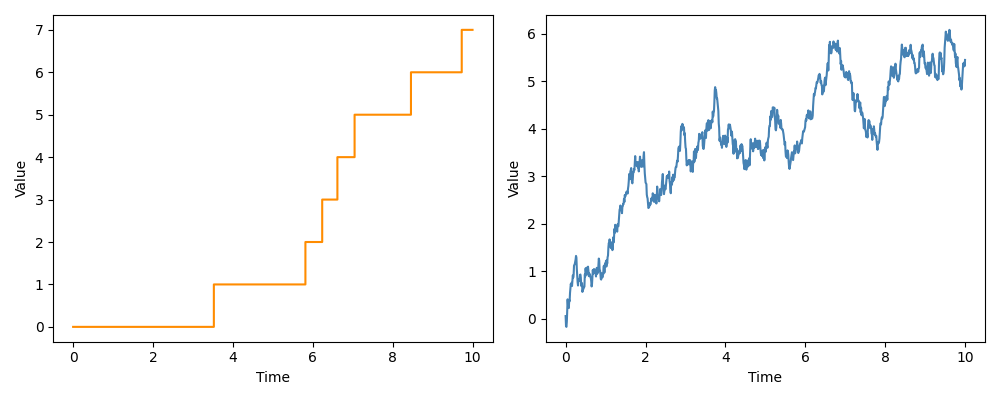
\includegraphics[width=0.8\textwidth]{./figures/1.png}
    \caption{Left: Poisson Process; Right: Brownian Motion.}
    \label{fig:poisson_brownian}
\end{figure}

\section{Filtration and Adaptedness}

\subsection{Definition of Filtration}

\begin{definition}[Filtration]
Let $(\Omega, \mathcal{F}, \mathbb{P})$ be a probability space. A family of $\sigma$-algebras $\{\mathcal{F}_t\}_{t \geq 0}$ is called a filtration if it satisfies:
\[
\mathcal{F}_s \subseteq \mathcal{F}_t \subseteq \mathcal{F}, \quad \forall s \leq t.
\]
\end{definition}

A filtration describes how information accumulates over time. Intuitively, $\mathcal{F}_t$ represents the collection of all random events observable up to time $t$. As time progresses, more information becomes available.

In practical analysis, we usually require filtrations to satisfy the \textit{usual conditions}:

- \textbf{Right-continuity:} $\mathcal{F}_t = \bigcap_{s > t} \mathcal{F}_s$;
- \textbf{Completeness:} $\mathcal{F}_0$ contains all $\mathbb{P}$-null sets.

\subsection{Adaptedness}

\begin{definition}[Adapted Process]
Let $\{X_t\}_{t \geq 0}$ be a stochastic process. It is said to be \textit{adapted} to the filtration $\{\mathcal{F}_t\}$ if for all $t \geq 0$, the random variable $X_t$ is $\mathcal{F}_t$-measurable.
\end{definition}

Adaptedness means that the value of the process at time $t$, $X_t$, is "knowable" at time $t$—that is, it does not depend on future information. In stochastic integration and SDEs, this condition is crucial because only non-anticipative processes are allowed as integrands or coefficients.

We are only allowed to integrate based on what has already occurred, not on future knowledge (so if you made a poor decision, don’t justify it by saying “It was just a coincidence” ). In the definition of Itô integrals, adaptedness is a fundamental requirement, which we will discuss in the next chapter.

\subsection{Natural Filtration and Predictability}

Natural filtration is one of the most commonly used filtrations in the study of stochastic processes. In most cases, we assume that the behavior of a process depends only on its own history, making the natural filtration a basic structure for describing the flow of information.

\begin{definition}[Natural Filtration]
Let $\{X_t\}_{t \geq 0}$ be a stochastic process. Its natural filtration is defined as:
\[
\mathcal{F}^X_t := \sigma(X_s : 0 \leq s \leq t),
\]
i.e., the smallest $\sigma$-algebra generated by all values of the process over the interval $[0, t]$. The collection $\{\mathcal{F}^X_t\}_{t \geq 0}$ forms an information structure that grows with time and describes the observable information from the process itself at each moment.
\end{definition}

For example, the Brownian motion $W_t$ is adapted to its natural filtration
\[
\mathcal{F}^W_t := \sigma(W_s : 0 \leq s \leq t),
\]
since the value of $W_t$ is entirely determined by its past trajectory.

Predictable processes are even more restrictive than adapted ones—they require that the value at each time $t$ can be determined strictly from earlier times. Such processes are important in the later definition of stochastic integrals because they ensure that the integrand does not depend on future information. In most applications, left-continuous adapted processes are predictable. Although we do not delve into integration in this chapter, understanding the basic notion of predictability helps in grasping the measurability requirements for integrands in the construction of Itô integrals.

\begin{definition}[Predictable Process]
Let $\{\mathcal{F}_t\}_{t \geq 0}$ be a filtration. A process $\{H_t\}_{t \geq 0}$ is called predictable (with respect to this filtration) if it is measurable with respect to the predictable $\sigma$-algebra $\mathcal{P}$ on $[0,\infty) \times \Omega$, where $\mathcal{P}$ is the smallest $\sigma$-algebra generated by:

\begin{itemize}
    \item all left-continuous adapted processes;
    \item all piecewise constant processes that take $\mathcal{F}_{t_i}$-measurable values on intervals of the form $(t_i, t_{i+1}]$.
\end{itemize}
\end{definition}

It is worth noting that while adapted processes already prohibit “peeking into the future,” predictable processes are even stricter: they do not allow decisions to be made even “at the current moment”—only strictly based on the past. 

For example, suppose you decide whether to bring an umbrella at time $t$ by observing the current weather. Then your decision rule $H_t$ depends on $\mathcal{F}_t$ and is merely adapted. But if you had to decide before time $t$ based only on past weather (i.e., measurable with respect to $\mathcal{F}_{t-}$), then $H_t$ would be predictable.

This may sound strange—why is it called “predictable” if it doesn’t predict the future? Here, “predictable” means that one can know in advance what the process will do—not in an intuitive, forecasting sense, but in the strict sense of being predetermined by past information. Quite the paradox!

\section{Construction of Brownian Motion}

Brownian motion serves as the fundamental driving term in stochastic differential equations (SDEs), and its theoretical foundation is built upon a well-defined probabilistic structure. To ensure that such a process truly exists within a probability space—and can be simulated, analyzed, and applied—we must construct Brownian motion systematically from multiple perspectives.

\subsection{Axiomatic Definition of Brownian Motion}

In Definition~2.4, we already presented the axiomatic definition of standard Brownian motion. It consists of four core properties: starting at zero, independent increments, Gaussian increments, and continuous sample paths. This model of “continuous yet unpredictable” random perturbations has paths that are continuous but non-differentiable; its increments follow a Gaussian distribution and are independent, while the time structure is stationary.

Here, we briefly review the four main axioms of Brownian motion and interpret their mathematical significance:

\begin{itemize}

    \item \textbf{Initial value at zero}: $W_0 = 0$

    This condition ensures that Brownian motion starts from a fixed point, maintaining temporal consistency. In simulation, modeling, or theoretical analysis, a well-defined initial value allows for standardized comparisons and normalization of sample paths.

    \item \textbf{Independent increments}: Increments over disjoint intervals are independent

    For any sequence of time points $0 \leq t_0 < t_1 < \cdots < t_n$, the increments $W_{t_1} - W_{t_0}, W_{t_2} - W_{t_1}, \dots$ are mutually independent. This expresses the "memoryless" property of Brownian motion—its evolution in each time interval is independent of the past.

    \item \textbf{Gaussian increments}: For any $s < t$, the increment $W_t - W_s \sim \mathcal{N}(0, t - s)$.

    This means the size of fluctuations over any time interval is normally distributed with variance proportional to the length of the interval, capturing the process's uniform volatility over time.

    \item \textbf{Continuous sample paths}: The paths are continuous almost surely

    For almost every $\omega \in \Omega$, the mapping $t \mapsto W_t(\omega)$ is continuous. Although the paths are continuous, Brownian motion is almost surely nowhere differentiable, which gives rise to its highly irregular trajectories. This structure is why Brownian motion effectively models "continuous but directionless" random perturbations.

\end{itemize}

\subsubsection{Path Continuity and Non-differentiability}

The sample paths of Brownian motion are continuous but almost surely non-differentiable. That is, even though there are no jumps in the trajectories and they appear smooth, the derivative is undefined at almost every point. This property distinguishes Brownian motion from many other stochastic processes.

\paragraph{Path Continuity}
Path continuity means that the sample path of the process does not abruptly break or jump over time. Mathematically, Brownian motion is right-continuous with no jumps over any finite time interval, almost surely. This stands in contrast to jump processes such as the Poisson process.

\paragraph{Non-differentiability}
Although Brownian motion paths are continuous, they lack well-defined derivatives at almost all time points—i.e., they are almost surely non-differentiable. This non-differentiability reflects the extreme irregularity of the paths and is mathematically tied to the roughness of the process. As the increments are random and fluctuations become increasingly frequent over time, the path lacks a stable derivative at any point.

\subsection{Covariance Structure and Gaussian Process}

One of the most important properties of Brownian motion is that it is a **Gaussian process**. This means that all of its finite-dimensional distributions are multivariate normal, and its covariance structure plays a central role. The covariance function of Brownian motion is:
\[
\mathbb{E}[W_s W_t] = \min(s, t)
\]
This tells us that the value of Brownian motion at any time depends not only on the current perturbation but also on historical information.

\paragraph{Gaussian Process}
A Gaussian process is defined by the property that every finite-dimensional distribution is a multivariate normal distribution. Brownian motion is a special case: for any collection of time points $t_1, t_2, \dots, t_n$, the joint distribution of $\{W_{t_i}\}$ is multivariate normal with zero mean and covariance given by $\mathbb{E}[W_s W_t] = \min(s, t)$. This implies that earlier values influence later changes, though the influence decays over time. It also implies that the increments are stationary—but still random.

The covariance structure of Brownian motion underpins its role in modeling stochastic processes. Moreover, the Gaussian nature makes it analytically tractable—properties of Gaussian processes (e.g., closure under linear operations, conditional distributions) make Brownian motion particularly convenient for many theoretical tools.

These properties describe the behavior of Brownian motion, but they do not yet guarantee its existence. In other words, although we have defined what Brownian motion should look like, we still need to construct a process on some probability space that satisfies these axioms.

\subsubsection*{Kolmogorov Existence Theorem}

To prove the existence of Brownian motion, we rely on the Kolmogorov Existence Theorem, which allows us to construct a stochastic process from a family of consistent finite-dimensional distributions. If a collection of finite-dimensional distributions satisfies certain consistency conditions—meaning that the joint distributions across different time points behave as expected—then a stochastic process exists whose finite-dimensional distributions match those specified.

\begin{theorem}[Kolmogorov Existence Theorem]
Let $\{F_t\}_{t \geq 0}$ be a family of finite-dimensional distributions satisfying consistency conditions. That is, for any $0 \leq s < t$, the joint distribution satisfies:
\[
\mathbb{P}(X_s \leq x_1, X_t \leq x_2) = \mathbb{P}(X_s \leq x_1) \cdot \mathbb{P}(X_t \leq x_2 \mid X_s = x_1).
\]
Then, there exists a probability space $(\Omega, \mathcal{F}, \mathbb{P})$ and a family of random variables $\{X_t\}_{t \geq 0}$ such that their finite-dimensional distributions agree exactly with $F_t$. In other words, a stochastic process exists that satisfies these distributional properties.
\end{theorem}

In constructing Brownian motion, we apply the Kolmogorov theorem to derive a stochastic process from its finite-dimensional distributions (i.e., the Gaussian distribution of increments over each time interval). By ensuring that the increments follow normal distributions and satisfy independence and stationarity, we can construct a process that satisfies all axioms of Brownian motion.

\subsection{Levy-Ciesielski Construction}

The Levy-Ciesielski construction provides a method for building Brownian motion from a discrete process. This method represents the continuous path of Brownian motion as the limit of discrete symmetric random walks, offering an elegant theoretical and numerical approach to constructing Brownian motion.

The construction is based on the wavelet expansion of Brownian motion paths. Suppose we have a collection of independent standard normal random variables $\{Z_k\}$, which represent the increments of a discrete process. By taking weighted sums of these increments and segmenting them over specific time intervals, we can build continuous Brownian motion paths. Brownian motion is viewed as the limit of infinitely many tiny steps, where each step is drawn from a discrete process such as a symmetric random walk. By appropriately scaling and weighting the increments, one generates a Brownian path.

Let $\{Z_k\}$ be a sequence of independent standard normal variables based on a binary wavelet basis. Then a Brownian path can be constructed via the following series expansion:
\[
W_t = \sum_{k=1}^{\infty} 2^{-\frac{k}{2}} Z_k \mathbf{1}_{[2^{-k}, 2^{-k+1})}(t),
\]
where $\{Z_k\}$ are i.i.d.\ $\mathcal{N}(0,1)$ and $\mathbf{1}_{[a,b)}(t)$ is the indicator function on the interval $[a, b)$.

Brownian motion is expressed as a linear combination of increments whose magnitude diminishes as $k$ increases. This method effectively treats Brownian motion as a discretized process of “infinite precision,” where each segment of perturbation contributes to a smooth trajectory in the limit.

A key advantage of the Levy-Ciesielski construction is that it builds a smooth continuous process from a discrete random walk while preserving all essential statistical properties of Brownian motion—independent increments, Gaussian distributions, and path continuity.

While mathematically elegant, the Levy-Ciesielski method may face computational limitations in practice. Especially for high-precision path generation, a large number of wavelet coefficients must be computed, which can be resource-intensive. Therefore, in practical numerical simulations, it is often combined with other approximation techniques.

\subsection{Donsker’s Theorem}

We may also take a different perspective on constructing Brownian motion by viewing it as the limit of discrete-time symmetric random walks. Donsker’s Theorem asserts that, under proper scaling, a discrete process such as a symmetric random walk converges in distribution to Brownian motion.

Let $\{S_n\}_{n \geq 0}$ be a properly scaled symmetric random walk (e.g., with step size $1/\sqrt{n}$ and each step being independent and uniformly distributed in direction). Then as $n \to \infty$, the path of this random walk converges to Brownian motion $W_t$:
\[
\lim_{n \to \infty} \frac{S_{\lfloor nt \rfloor}}{\sqrt{n}} = W_t.
\]
Here, $S_n$ denotes the discrete-time random walk, and $\lfloor nt \rfloor$ denotes the index at time $t$. Donsker’s Theorem thus provides a convergence result for discrete processes toward continuous Brownian motion.

It is important to note that this is a statement of convergence: as the time intervals become infinitesimally small and the number of steps grows, the trajectory of the discrete process approaches a continuous path whose increments follow a normal distribution.

Donsker’s Theorem not only lays the theoretical foundation for Brownian motion but also plays a central role in practical applications such as numerical simulation and approximation of stochastic processes. It allows us to simulate Brownian motion using discrete random walks and approximate trajectories by increasing the time resolution. Together with the Levy-Ciesielski construction, it finds wide application in numerical solutions of stochastic differential equations.

\end{document}
